\documentclass[fleqn,10pt,lineno]{wlpeerj}

\usepackage{amsmath}
\usepackage{amssymb}
\usepackage{booktabs}
\usepackage{multirow}
\usepackage{placeins}
\usepackage{float}
\usepackage{flafter}
\usepackage{microtype}
\usepackage{url}
\usepackage[authoryear,round]{natbib}
\usepackage{hyperref}
\hypersetup{colorlinks=true,linkcolor=blue,citecolor=blue,urlcolor=blue}
\usepackage{graphicx}
\usepackage{iftex}

\ifPDFTeX
\else
  \usepackage{fontspec}
  \setmainfont{TeX Gyre Termes}
  \setsansfont{TeX Gyre Heros}
  \setmonofont{Latin Modern Mono}
\fi

\let\cite\citep

\graphicspath{{../../}{../../figures/}{figures/}}

\setlength{\textfloatsep}{8pt plus 2pt minus 2pt}
\setlength{\floatsep}{8pt plus 2pt minus 2pt}
\setlength{\intextsep}{8pt plus 2pt minus 2pt}
\setlength{\abovecaptionskip}{4pt}
\setlength{\belowcaptionskip}{2pt}
\renewcommand{\arraystretch}{0.95}
\renewcommand{\topfraction}{0.9}
\renewcommand{\bottomfraction}{0.8}
\renewcommand{\textfraction}{0.08}
\renewcommand{\floatpagefraction}{0.8}

\title{Matrix-Residual Graph Neural Networks for Graph Classification}

\author[1]{Xuelin Hu}
\author[2]{Xiaoqin Fu}

\affil[1]{School of Railway Communication and Signaling Engineering, Liuzhou Railway Vocational Technical College, Liuzhou 545000, China}
\affil[2]{School of Railway Locomotive and Rolling Stock, Liuzhou Railway Vocational Technical College, Liuzhou 545000, China}

\corrauthor[2]{Xiaoqin Fu}{fuxiaoqin@ltzy.edu.cn}

\begin{abstract}
\textbf{Background.} Residual connections are widely used to stabilize graph neural networks, but residual design is often treated as a one-dimensional depth-wise choice. Multi-branch graph classifiers create a richer design space: residual information can flow along depth, across branches, or through a local two-dimensional branch-by-layer neighborhood.

\textbf{Methods.} We study Matrix-Residual Graph Neural Networks as a controlled residual-topology framework for graph classification. The model family represents hidden states on a branch-by-layer grid and compares five information-flow designs: plain message passing, vertical residual reuse, horizontal branch-wise exchange, local matrix residual reuse, and sparse/gated matrix reuse. The main benchmark evaluates six datasets, four message-passing operators, five model families, and five graph-level folds under a shared training protocol. We further run branch-count ablations, fold-0 sensitivity scans, five-fold checks of selected MatrixResGated candidates, and mechanism analyses. To further test effectiveness across structural granularities, we construct a controlled synthetic multi-class benchmark spanning five graph families and two to eight structural classes.

\textbf{Results.} Real-data experiments show that no single residual topology is universally optimal across datasets and operators. Branch-count ablations reveal dataset-dependent operating regions rather than monotonic capacity gains. The synthetic multi-class benchmark further shows that simple baselines remain competitive on low-class tasks, whereas MatrixRes and MatrixResGated become more consistently favorable as structural class granularity increases.

\textbf{Conclusions.} Residual topology, branch count, and residual filtering should be selected jointly. Additional branches help only when they create useful functional diversity; otherwise, residual traffic and branch redundancy can offset the added capacity. Matrix-style reuse is best understood as a tunable residual family rather than a universal replacement for simpler vertical or horizontal residual paths, with its clearest advantage appearing under finer-grained structural discrimination.
\end{abstract}

\begin{document}

\flushbottom
\maketitle
\thispagestyle{empty}
\noindent\textbf{Keywords:} Graph classification; Graph neural networks; Residual connections; Multi-branch architectures; Matrix residual reuse; Synthetic graph benchmarks
\par\medskip

\section{Introduction}

Graph neural networks (GNNs) learn graph representations by repeatedly aggregating information from local neighborhoods \cite{gori2005new,kipf2017gcn}. This message-passing view has become a standard tool for graph classification because it combines node attributes, local connectivity, and graph-level structure in a single differentiable model \cite{gilmer2017neural,wu2020comprehensive}. In molecular and protein-oriented benchmarks, graph labels may depend on both local motifs and global organization, so useful intermediate evidence must survive until graph-level pooling \cite{duvenaud2015convolutional,ying2018hierarchical}.

Increasing depth or adding parallel branches can expand model capacity, but it also changes information transport through the network. Deep GNNs may suffer from over-smoothing, where node representations become too similar across propagation steps \cite{li2018deeper,oono2020simple}. They may also suffer from over-squashing, where long-range information is compressed into limited-size messages \cite{alon2020bottleneck,topping2021understanding}. These issues are especially relevant for graph-level prediction because the final readout depends on the quality of the intermediate representations that reach the pooling stage.

Residual connections are a common response to these difficulties. They improve gradient flow and allow earlier representations to be reused, a principle established in deep convolutional networks and later adapted to graph architectures \cite{he2016deep,bresson2017residual}. Other depth-control strategies, including DropEdge, Jumping Knowledge aggregation, and graph-specific normalization, also aim to preserve useful information across propagation steps \cite{rong2019dropedge,xu2018representation}. However, residual connectivity is still commonly treated as a default layer-wise component rather than as the object of study. Most residual graph classifiers reuse information along depth in the same stream.

Once a model contains multiple branches, depth-wise residual reuse is only one possible route. Residual information may also move across neighboring branches at the same depth or through diagonal branch-depth neighborhoods. Existing graph-classification work has explored stronger message-passing operators, hierarchical pooling, attention, and higher-order neighborhood mixing \cite{abu2019mixhop,bianchi2020graph}. These designs improve the expressive or aggregation capacity of GNNs, but they do not isolate the residual-routing question: if several branch states are available at a given depth, should the model reuse only the previous state of the same branch, exchange states laterally, or combine both directions in a local two-dimensional residual neighborhood?

This paper studies residual reuse as a structured design problem on a branch-by-layer grid. The central question is not whether skip connections should be present, but where residual signals should flow. A grid view exposes three controlled neighborhoods: vertical reuse along depth, horizontal exchange across neighboring branches, and matrix-style reuse that combines same-branch, neighboring-branch, and diagonal residual paths. A sparse/gated matrix variant further tests whether matrix residual traffic should be filtered before injection. This framing follows controlled benchmark practice: the goal is not to add many unrelated architectural components, but to make one design axis explicit enough to evaluate \cite{keriven2020benchmark,morris2020tudataset}.

The study is deliberately controlled. It fixes the graph-classification pipeline within each comparison, evaluates the same architecture family under several canonical message-passing operators, and changes only the residual topology and residual-control mechanism. This separation keeps the empirical comparison focused on information-flow design rather than on unrelated changes in readout structure, task-specific feature engineering, or operator-specific tuning. Recent graph models may achieve stronger absolute performance by changing several components simultaneously; here, those components are intentionally held fixed so that the residual topology itself remains identifiable.

Real graph benchmarks are also limited in the range of structural class granularity that they expose. A residual topology may look adequate on binary graph classification while behaving differently when the label space requires finer structural separation. To test this point without adding task-specific feature engineering, we complement the real-data benchmark with controlled synthetic graph families whose class labels are generated by structural parameters. This synthetic setting is not intended to replace real benchmarks; it is a stress test for whether residual routing remains stable as structural classes become more fine-grained.

The work is organized around three research questions:
\begin{enumerate}
    \item \textbf{Does residual topology affect performance under a shared graph-classification protocol?} We compare plain message passing, vertical residual reuse, horizontal branch-wise exchange, local matrix residual reuse, and sparse/gated matrix reuse while holding the remaining pipeline fixed.
    \item \textbf{How do branch count, residual traffic, and mechanisms explain performance changes?} We test whether additional branches improve accuracy monotonically or only within a useful operating region, and we relate these trends to diversity, similarity, gradients, and residual traffic.
    \item \textbf{When is matrix-style residual reuse more effective on real data and controlled synthetic multi-class structures?} We test whether matrix residual traffic should be passed densely or filtered, whether candidate residual-control settings remain valid after full-fold reruns, and whether matrix-style reuse becomes more stable as structural class granularity increases.
\end{enumerate}

The main contributions are:
\begin{itemize}
    \item \textbf{A branch-by-layer formulation of residual graph classifiers.} Vertical, horizontal, matrix, and sparse/gated matrix residual families are expressed as local neighborhoods on the same grid, making their information-flow differences explicit.
    \item \textbf{A controlled real-data benchmark and synthetic multi-class benchmark.} The experiments keep the classifier, readout, fold protocol, and backbone choices matched, and add a structural stress test spanning five controlled graph families and two to eight classes.
    \item \textbf{A mechanism analysis with conservative rerun checks.} Accuracy is analyzed together with branch diversity, branch cosine similarity, branch CKA, gradient norms, and residual activity. Sensitivity scans are used only to identify candidates, and selected settings are rerun across folds before being treated as empirical evidence.
\end{itemize}

\section{Materials and Methods}
\label{sec:methods}

This section defines the graph-classification task, the Matrix-Residual architecture family, the benchmark protocol, the synthetic structural stress test, and the mechanism metrics. The guiding principle is to isolate residual topology while holding the remaining learning pipeline fixed.

\subsection{Problem definition and notation}

Let \(\mathcal{G}=(\mathcal{V},\mathcal{E})\) be a graph with node feature matrix \(\mathbf{X}\in\mathbb{R}^{n\times d_{\mathrm{in}}}\) and adjacency structure \(\mathbf{A}\). For a dataset \(\mathcal{D}=\{(\mathcal{G}_i,y_i)\}_{i=1}^{N}\), the objective is to learn \(f_{\theta}:\mathcal{G}\rightarrow \hat{y}\), where \(\hat{y}\) is the predicted graph label.

The compared model families share the same graph-classification wrapper:
\begin{itemize}
    \item \textbf{Plain}: stacked message passing without explicit residual reuse.
    \item \textbf{VerticalRes}: same-branch residual reuse from the previous layer.
    \item \textbf{HorizontalRes}: cross-branch exchange between adjacent branches at the same depth.
    \item \textbf{MatrixRes}: local two-dimensional reuse over vertical, horizontal, and diagonal neighbors.
    \item \textbf{MatrixResGated}: matrix reuse with gated or sparse residual filtering.
\end{itemize}

\subsection{Shared graph-classification pipeline}

Let \(B\) be the number of branches and \(L\) be the number of message-passing layers. The hidden state at branch \(b\) and layer \(\ell\) is written as \(\mathbf{H}^{(\ell)}_{b}\), where \(b\in\{1,\ldots,B\}\). A branch-local propagation step is
\begin{equation}
\mathbf{Z}^{(\ell)}_{b} = \phi^{(\ell)}_{b}\left(\mathbf{H}^{(\ell-1)}_{b}, \mathbf{A}\right),
\end{equation}
where \(\phi\) is instantiated as one of four standard operators: GCNConv \cite{kipf2017gcn}, GATConv \cite{velivckovic2017graph}, SAGEConv \cite{hamilton2017inductive}, or GINConv \cite{xu2019gin}. The residual-enhanced update is
\begin{equation}
\mathbf{H}^{(\ell)}_{b} =
\mathbf{Z}^{(\ell)}_{b} +
\sum_{(b',\ell')\in\mathcal{N}(b,\ell)}
\mathcal{R}_{(b',\ell')\rightarrow(b,\ell)}
\left(\mathbf{H}^{(\ell')}_{b'}\right).
\end{equation}
The only term that changes across architectures is the residual neighborhood \(\mathcal{N}(b,\ell)\) and the residual transform \(\mathcal{R}\).

After the final message-passing layer, each branch is pooled to a graph-level vector by global mean pooling and the branch vectors are combined before classification. We intentionally avoid architecture-specific pooling heads such as differentiable pooling or self-attention pooling \cite{ying2018hierarchical,lee2019self}, because the purpose is to isolate residual topology rather than to compare readout mechanisms. The classifier is trained with cross-entropy loss. Figure~\ref{fig:architecture} summarizes the shared pipeline and the residual routes compared in the study.

\begin{figure}[!htbp]
\centering
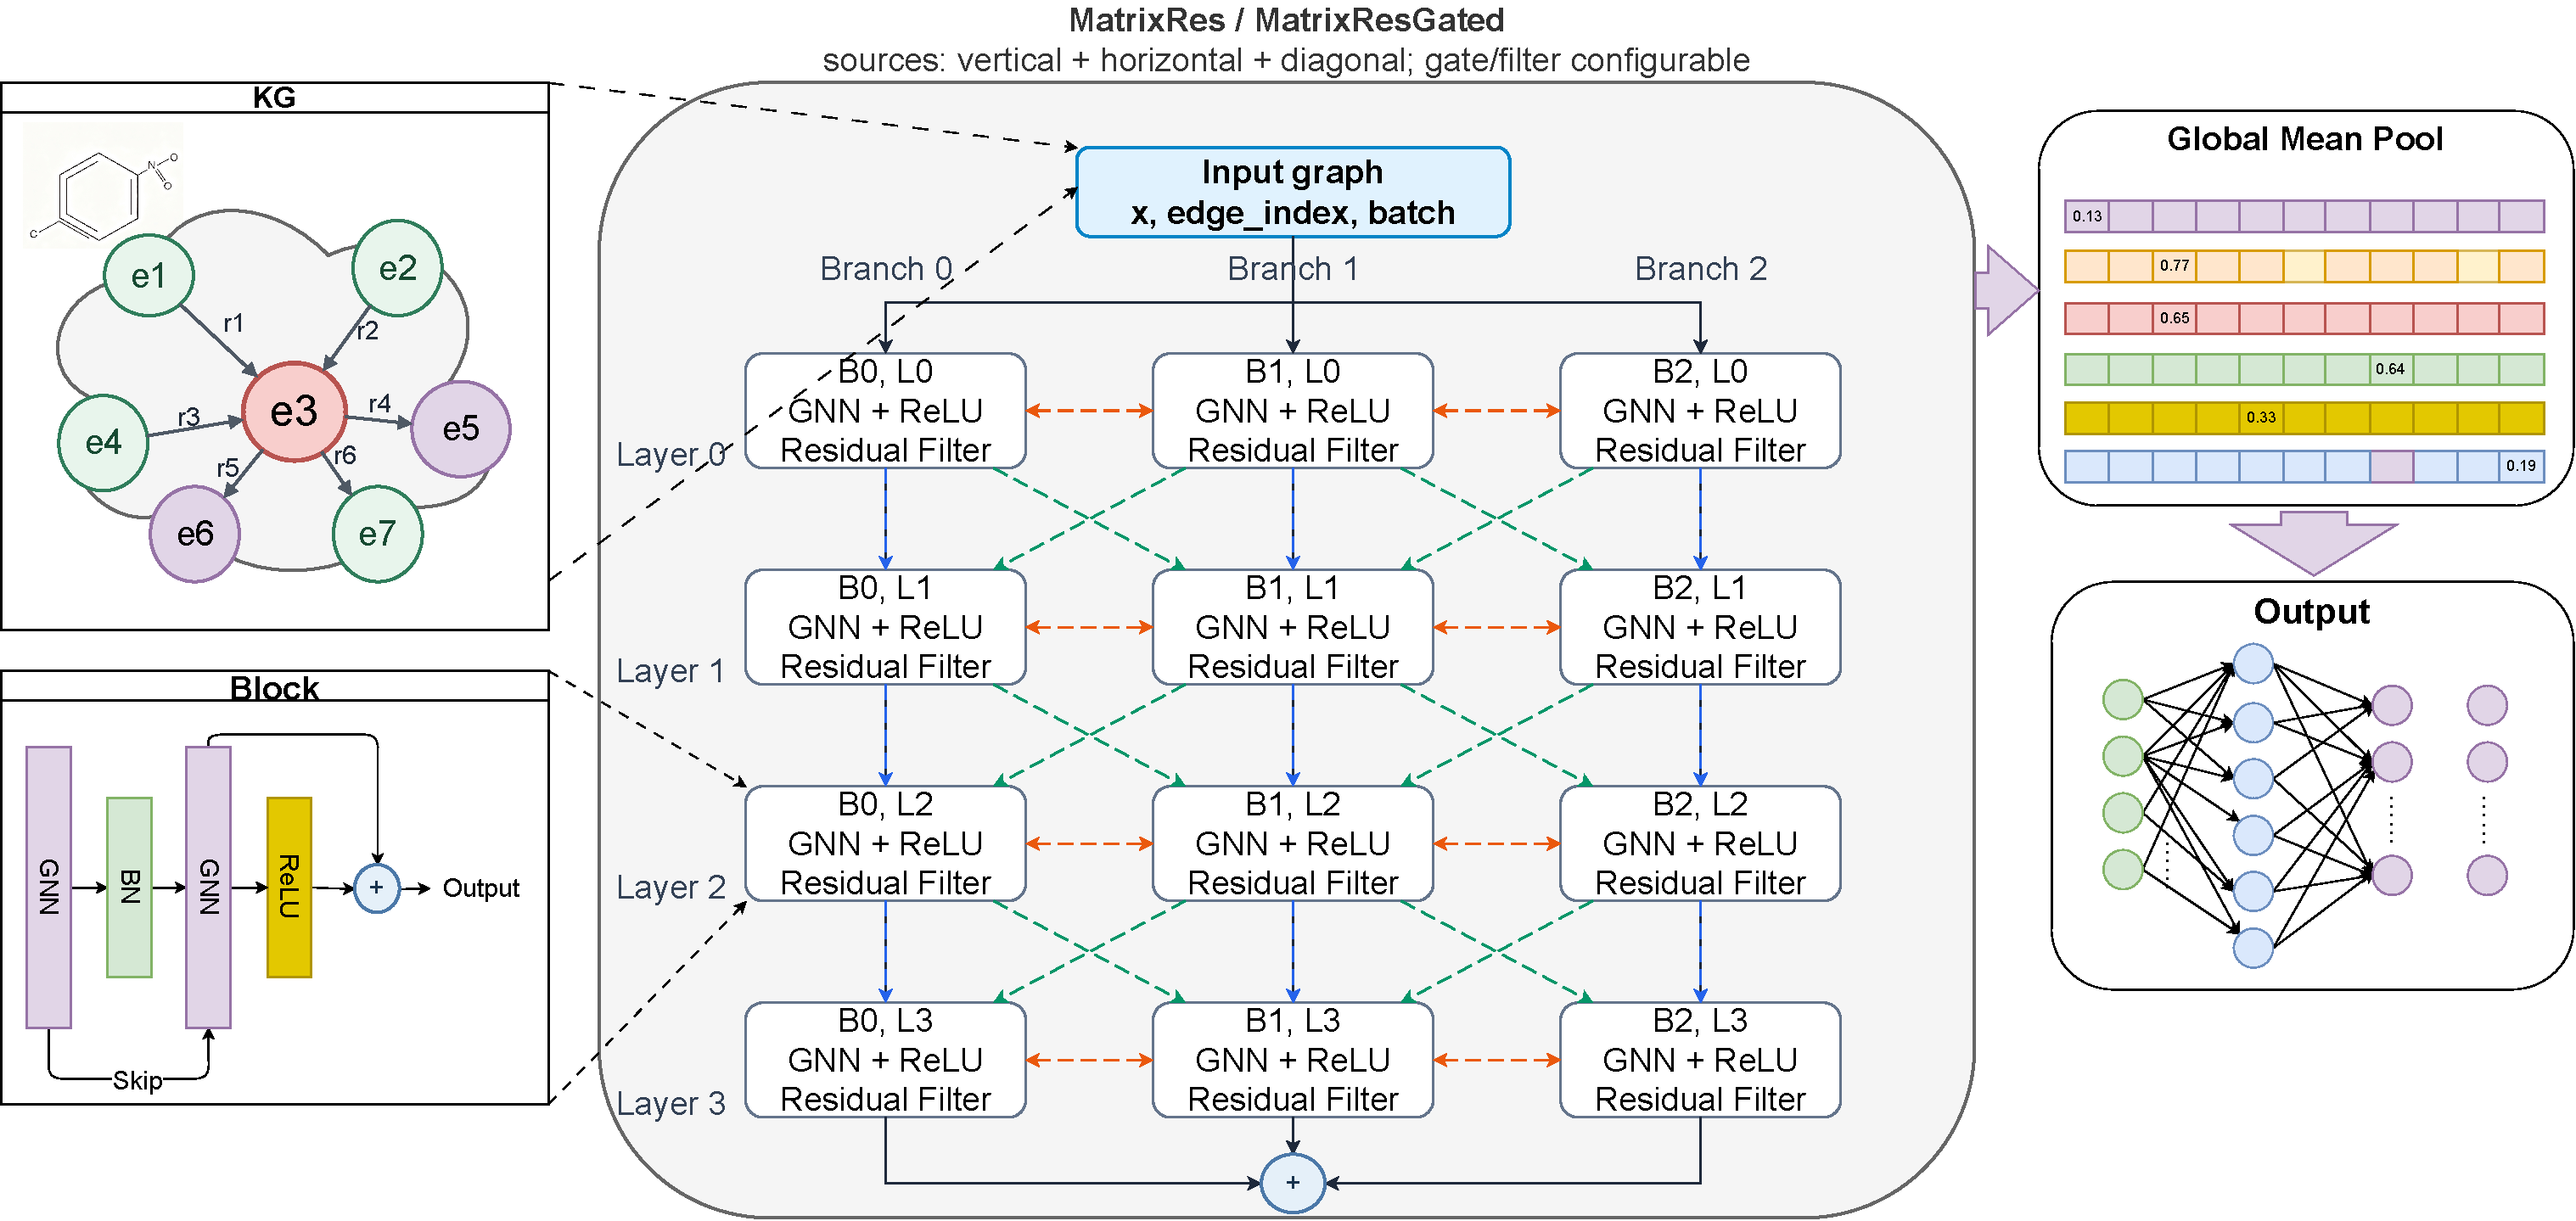
\includegraphics[width=0.95\linewidth]{figures/cr_gnn_graph_architecture.pdf}
\caption{Architecture overview of the compared residual neighborhoods on the branch-by-layer grid. The same message-passing backbone and graph-level readout are kept fixed while the residual routes are changed.}
\label{fig:architecture}
\end{figure}

\subsection{Residual neighborhoods}
\label{sec:model}

\textbf{Plain.} The plain baseline has no residual neighborhood:
\begin{equation}
\mathcal{N}(b,\ell)=\emptyset.
\end{equation}

\textbf{VerticalRes.} Vertical residual reuse injects the previous layer on the same branch:
\begin{equation}
\mathcal{N}(b,\ell)=\{(b,\ell-1)\}.
\end{equation}

\textbf{HorizontalRes.} Horizontal residual reuse exchanges information across adjacent branches at the same depth:
\begin{equation}
\mathcal{N}(b,\ell)=\{(b-1,\ell),(b+1,\ell)\},
\end{equation}
with boundary branches using only valid neighbors. When \(B=1\), this horizontal neighborhood is empty.

\textbf{MatrixRes.} Matrix residual reuse combines vertical, horizontal, and diagonal neighborhoods:
\begin{equation}
\mathcal{N}(b,\ell)=
\{(b,\ell-1),(b-1,\ell),(b+1,\ell),(b-1,\ell-1),(b+1,\ell-1)\}.
\end{equation}
This local stencil is intentionally not dense all-to-all mixing. It preserves an interpretable residual structure over the branch-by-layer grid. Invalid boundary neighbors are removed; therefore, when \(B=1\), MatrixRes keeps the same-branch vertical residual path after the first layer but has no branch-neighbor routes.

\textbf{MatrixResGated.} MatrixResGated uses the same neighborhood as MatrixRes, but the residual transform controls the injected signal:
\begin{equation}
\mathcal{R}(\mathbf{U}) =
\begin{cases}
\alpha \mathbf{U}, & \text{identity residual filtering with a gate},\\
\alpha\,\mathrm{softshrink}_{\lambda}(\mathbf{U}), & \text{sparse residual filtering with a gate}.
\end{cases}
\end{equation}
In the main benchmark, Plain, VerticalRes, HorizontalRes, and MatrixRes use identity residual filtering. MatrixResGated uses sparse residual filtering with \(\lambda=0.05\) and a learnable scalar gate initialized at 0.8. When \(B=1\), MatrixResGated still applies gated sparse filtering to the remaining matrix-residual paths. The implementation also supports top-\(k\) residual filtering and fixed gates, but these are not the default settings used for the main reported results.

\subsection{Datasets and sources}
\label{sec:datasets}

The main benchmark uses six third-party datasets from TUDataset \cite{morris2020tudataset}: PROTEINS, DD, ENZYMES, MUTAG, AIDS, and Mutagenicity. The TUDataset collection is available at \url{https://chrsmrrs.github.io/datasets/} and is accessed through PyTorch Geometric \cite{fey2019fast}. PROTEINS and DD are binary protein-structure graph classification benchmarks, ENZYMES is a six-class enzyme classification benchmark, and MUTAG, AIDS, and Mutagenicity provide supplementary molecular-graph robustness checks. All experiments use the raw benchmark features and graph structures without task-specific feature engineering, graph augmentation, or edge redesign.

\subsection{Data preprocessing}

The preprocessing pipeline is intentionally minimal to keep the comparison focused on residual topology. TUDataset graphs are loaded with their provided node features and graph labels. The code does not add handcrafted chemical or biological descriptors, does not perform graph augmentation, and does not rewire edges. Synthetic graphs are generated from controlled structural parameters, assigned generic eight-dimensional node features derived from normalized degree and random feature channels, and then passed to the same graph-classification pipeline. For every dataset, graph-level folds are fixed by the experiment scripts so that all compared residual topologies use matched train, validation, and test splits.

\subsection{Technique selection}

The implemented techniques were selected to isolate one architectural factor: residual information flow in a multi-branch GNN. GCNConv, GATConv, SAGEConv, and GINConv were chosen because they are canonical message-passing operators representing spectral-style convolution, attention-based aggregation, neighborhood sampling/aggregation, and injective multiset aggregation. Plain, VerticalRes, HorizontalRes, MatrixRes, and MatrixResGated were then compared under the same operators, pooling, classifier, and fold protocol. This selection makes the residual-topology question testable without mixing it with unrelated changes in readout design, feature engineering, or task-specific model tuning.

\subsection{Evaluation protocol and metrics}

All main results use graph-level five-fold evaluation. For fold \(k\), the test accuracy is
\begin{equation}
\mathrm{Acc}_{k}=
\frac{1}{|\mathcal{T}_{k}|}
\sum_{(\mathcal{G}_{i},y_{i})\in\mathcal{T}_{k}}
\mathbf{1}[\hat{y}_{i}=y_{i}].
\end{equation}
Across folds, we report
\begin{equation}
\overline{\mathrm{Acc}}=\frac{1}{5}\sum_{k=1}^{5}\mathrm{Acc}_{k},
\end{equation}
and the fold-level standard deviation.

Accuracy is the primary metric because every benchmark is a graph-level classification task with discrete labels and because it is the standard summary reported for the selected TUDataset tasks. The fold-level standard deviation is reported to expose variability across train/test splits. For the synthetic multi-class benchmark, macro-F1 is added because it gives equal weight to each class, and chance-normalized accuracy is added because raw accuracy is not directly comparable when the number of classes changes from two to eight. Mechanism metrics such as branch diversity, cosine similarity, CKA, residual activity, and gradient norm are used as diagnostic measurements rather than as optimization targets.

\subsection{Synthetic multi-class structural benchmark}
\label{sec:synthetic}

To test residual topology under controlled structural class granularity, we add a synthetic benchmark based on five graph families: Bernoulli random graphs recorded as ER, Barabási--Albert (BA) graphs, stochastic block models (SBM), Watts--Strogatz (WS) graphs, and a regular-degree control. For each family, we generate seven multi-class datasets with class counts \(C\in\{2,3,4,5,6,7,8\}\). Each class contains 200 graphs, so each dataset contains \(200C\) graphs. Graph sizes are sampled between 30 and 80 nodes, and every node receives an eight-dimensional feature vector derived from normalized degree and random feature channels. The features are intentionally generic and do not encode the class label directly.

The synthetic labels are controlled by family-specific structural parameters. The ER identifier in our experiment records corresponds strictly to Gilbert's \(G(n,p)\) model: each node pair is connected independently with Bernoulli probability \(p\), producing sparse random structures at different densities \cite{gilbert1959random}. BA classes differ by the preferential-attachment count and provide long-tailed degree structures \cite{barabasi1999emergence}. SBM classes vary the within-block and between-block probabilities to control community separation \cite{holland1983stochastic}. WS classes differ by rewiring probability and provide small-world structures with local clustering and short paths \cite{watts1998collective}. The regular-degree control uses randomly relabeled regular ring lattices with different fixed degrees. It provides degree-uniform structures but is not sampled from the uniform random-regular distribution, for which \cite{wormald1999models} provides background. These families are used as stress tests rather than as replacements for real graph-classification benchmarks.

The synthetic benchmark uses the same five model families, four message-passing operators, branch count \(B=3\), and five-fold protocol as the main benchmark, producing 35 datasets and 3,500 completed model runs. Because accuracy values are not directly comparable across different class counts, we report macro-F1 and chance-normalized accuracy in addition to raw accuracy. For a \(C\)-class dataset, normalized accuracy is
\begin{equation}
\mathrm{NAcc}=\frac{\mathrm{Acc}-1/C}{1-1/C}.
\end{equation}
This metric maps chance-level accuracy to 0 and perfect accuracy to 1, making the two- to eight-class scaling trend easier to interpret.

\subsection{Training configuration}

All main benchmark runs use the default branch count \(B=3\). The benchmark is repeated under four message-passing operators: GCNConv, GATConv, SAGEConv, and GINConv. The hidden dimension is 64 unless a sensitivity setting changes it. The default depth is \(L=4\) message-passing layers, except DD, where \(L=3\) is used for the main benchmark. All models use ReLU nonlinearities and the default PyTorch/PyTorch Geometric parameter initialization for the corresponding layers. Models are optimized with Adam \cite{kingma2014adam}; the checkpoint with the lowest validation loss is retained for test evaluation. Early stopping monitors validation loss, and all runs use ReduceLROnPlateau with factor 0.5, patience 15, and minimum learning rate \(10^{-5}\). Gradients are clipped at norm 2.0. The branch-count ablation evaluates \(B=1,\ldots,8\) for HorizontalRes, MatrixRes, and MatrixResGated on PROTEINS and DD under GCNConv. The sensitivity scan evaluates MatrixRes and MatrixResGated on fold 0 at \(B=3\), varying learning rate, dropout, hidden dimension, sparsity strength, and gate initialization. Selected MatrixResGated candidates are then rerun across all five folds.

\begin{table}[!htbp]
\centering
\small
\caption{Key experimental settings shared by the main benchmark.}
\label{tab:hyperparams}
\begin{tabular}{l p{0.62\linewidth}}
\toprule
Parameter & Value \\
\midrule
Message-passing operators & GCNConv, GATConv, SAGEConv, GINConv \\
Default branch count & 3 \\
Default layers & 4, except DD uses 3 \\
Default hidden dimension & 64 \\
Evaluation & Five-fold graph classification \\
Synthetic stress test & ER, BA, SBM, WS, and regular-degree controls with \(C=2,\ldots,8\), 200 graphs per class \\
Branch-count ablation & \(B=1,\ldots,8\) \\
Primary metrics & Mean best test accuracy; synthetic benchmark also reports macro-F1 and normalized accuracy \\
Sensitivity scope & Fold 0, \(B=3\) \\
Plain/VerticalRes/HorizontalRes & 200 epochs, patience 60, learning rate 0.005, weight decay \(10^{-4}\), dropout 0.5 \\
MatrixRes/MatrixResGated & 240 epochs, patience 80, learning rate 0.003, weight decay \(5\times10^{-5}\), dropout 0.3 \\
Dataset-specific settings & DD uses dropout 0.3; ENZYMES uses batch size 128 \\
Learning-rate schedule & ReduceLROnPlateau, factor 0.5, patience 15, min lr \(10^{-5}\) \\
Gradient clipping & Norm 2.0 \\
\bottomrule
\end{tabular}
\end{table}

\subsection{Computing infrastructure}

The experiments were run on an Ubuntu Linux x86\_64 server equipped with an AMD Ryzen 7 5700X CPU with 8 physical cores and 16 threads, and an NVIDIA GeForce RTX 3090 GPU with 24 GB of memory. The NVIDIA driver version was 580.126.09 and reported CUDA 13.0 support through \texttt{nvidia-smi}; the CUDA compiler \texttt{nvcc} was not available in the runtime environment. The server-side Python version was 3.13.12. The repository stores the scripts, configuration files, frozen logs, generated figures, and supporting evidence needed to audit the reported experiments.

\subsection{Mechanism metrics}

To interpret branch-count behavior, we track several mechanism indicators on the final branch-level graph embeddings. Branch diversity is the mean pairwise Euclidean distance between branch embeddings. Branch cosine similarity is the mean pairwise cosine similarity, and branch CKA is linear centered-kernel alignment computed on the same branch-embedding set. For \(B=1\), there is no branch pair; we report diversity as 0 and cosine and CKA as 1 under the single-branch self-similarity convention. Mean gradient norm is the representative parameter-gradient norm recorded during training. Residual-count totals summarize how many residual inputs are available across residual sites, active ratio measures the fraction of nonzero residual entries after filtering, and the gate statistic reports the learned scalar gate used by MatrixResGated. These metrics are used as correlational diagnostics rather than as causal tests.

\section{Results and Discussion}
\label{sec:results}

All results are reported as five-fold mean best test accuracy \(\pm\) fold-level standard deviation unless otherwise stated.

\subsection{Overall benchmark performance}

The main benchmark asks whether residual topology has a stable winner across datasets and message-passing operators. It does not. Table~\ref{tab:operator_wins} summarizes the full benchmark: across the 24 dataset--operator combinations, MatrixRes is the most frequent winner, with 9 wins and the best mean rank (2.12). MatrixResGated and Plain each win 5 combinations, HorizontalRes wins 3, and VerticalRes wins 2. Thus, matrix-style reuse has the most favorable aggregate profile in this controlled benchmark, but every topology has a setting in which it is the strongest choice.

\begin{table}[!htbp]
\centering
\small
\caption{Winner counts and mean ranks across the 24 dataset--operator combinations. Lower mean rank is better.}
\label{tab:operator_wins}
\begin{tabular}{l c c l}
\toprule
Model & Wins & Mean rank & Interpretation \\
\midrule
Plain & 5 & 3.04 & Strong on selected small or easier settings \\
VerticalRes & 2 & 3.38 & Depth-only reuse helps selectively \\
HorizontalRes & 3 & 3.54 & Competitive when lateral exchange is sufficient \\
MatrixRes & \(\mathbf{9}\) & \(\mathbf{2.12}\) & Most frequent winner in this benchmark \\
MatrixResGated & 5 & 2.92 & Useful when sparse control helps residual traffic \\
\bottomrule
\end{tabular}
\end{table}

\begin{figure}[!htbp]
\centering
\includegraphics[width=0.82\linewidth]{figures/exp/fig_model_win_counts.pdf}
\caption{Model-level winner counts across the 24 dataset--operator combinations.}
\label{fig:model_win_counts}
\end{figure}

Table~\ref{tab:winners_by_operator} gives the cell-level evidence behind the win counts in Table~\ref{tab:operator_wins}. The matrix family is most prominent on MUTAG, AIDS, and Mutagenicity, where MatrixRes or MatrixResGated wins most operator settings. The protein-oriented datasets are more mixed: PROTEINS alternates between Plain and HorizontalRes, while DD alternates among HorizontalRes, MatrixRes, and VerticalRes. ENZYMES remains difficult and does not produce a stable residual-topology preference.

\begin{table}[!htbp]
\centering
\scriptsize
\caption{Winning model for each dataset and message-passing operator. Values in parentheses are mean best test accuracy.}
\label{tab:winners_by_operator}
\resizebox{\linewidth}{!}{%
\begin{tabular}{l c c c c}
\toprule
Dataset & GCNConv & GATConv & SAGEConv & GINConv \\
\midrule
PROTEINS & Plain (0.7044) & HorizontalRes (0.7116) & Plain (0.6999) & HorizontalRes (0.7080) \\
DD & HorizontalRes (0.7181) & MatrixRes (0.7164) & MatrixRes (0.7198) & VerticalRes (0.7224) \\
ENZYMES & MatrixResGated (0.2933) & Plain (0.2717) & VerticalRes (0.2883) & Plain (0.3100) \\
MUTAG & MatrixRes (0.7609) & MatrixResGated (0.7555) & MatrixRes (0.7504) & MatrixResGated (0.8081) \\
AIDS & MatrixRes (0.8365) & MatrixRes (0.8875) & Plain (0.8850) & MatrixResGated (0.9280) \\
Mutagenicity & MatrixRes (0.7784) & MatrixRes (0.7909) & MatrixResGated (0.8031) & MatrixRes (0.8024) \\
\bottomrule
\end{tabular}
}
\end{table}

The ENZYMES outcomes should be interpreted cautiously because the absolute accuracies are low for all compared models. Keeping ENZYMES in the full 24-combination summary preserves the preregistered benchmark scope, but it should not be read as strong evidence for a residual topology by itself. Excluding ENZYMES leaves MatrixRes with 9 wins across 20 dataset--operator combinations and a mean rank of 2.05, so the aggregate MatrixRes preference remains. The split is still context-dependent: MatrixRes is most prominent on the molecular datasets, whereas the protein-oriented datasets produce mixed winners.

\subsection{GCNConv benchmark slice}

To further remove variation caused by message-passing operators and observe the effect of residual topology under a fixed backbone, we report the GCNConv slice separately. Table~\ref{tab:main_benchmark} gives the full slice at the default branch count \(B=3\). Plain is strongest on PROTEINS, HorizontalRes is strongest on DD, MatrixResGated is strongest on ENZYMES, and MatrixRes is strongest on MUTAG, AIDS, and Mutagenicity.

\begin{table}[!htbp]
\centering
\scriptsize
\caption{GCNConv benchmark results with default branch count \(B=3\).}
\label{tab:main_benchmark}
\begin{tabular}{l c c c c c}
\toprule
Dataset & Plain & VerticalRes & HorizontalRes & MatrixRes & MatrixResGated \\
\midrule
PROTEINS & \(\mathbf{0.7044\pm0.0387}\) & \(0.6993\pm0.0340\) & \(0.6992\pm0.0399\) & \(0.6973\pm0.0324\) & \(0.6886\pm0.0397\) \\
DD & \(0.7053\pm0.0517\) & \(0.7143\pm0.0260\) & \(\mathbf{0.7181\pm0.0296}\) & \(0.7127\pm0.0365\) & \(0.7141\pm0.0359\) \\
ENZYMES & \(0.2683\pm0.0343\) & \(0.2550\pm0.0455\) & \(0.2633\pm0.0584\) & \(0.2750\pm0.0577\) & \(\mathbf{0.2933\pm0.0470}\) \\
MUTAG & \(0.7556\pm0.0439\) & \(0.7451\pm0.0695\) & \(0.7343\pm0.0433\) & \(\mathbf{0.7609\pm0.0715}\) & \(0.7556\pm0.0721\) \\
AIDS & \(0.8215\pm0.0046\) & \(0.8210\pm0.0233\) & \(0.8130\pm0.0297\) & \(\mathbf{0.8365\pm0.0412}\) & \(0.8150\pm0.0231\) \\
Mutagenicity & \(0.7644\pm0.0188\) & \(0.7667\pm0.0212\) & \(0.7738\pm0.0134\) & \(\mathbf{0.7784\pm0.0185}\) & \(0.7701\pm0.0165\) \\
\bottomrule
\end{tabular}
\end{table}

\begin{figure}[!htbp]
\centering
\includegraphics[width=0.92\linewidth]{figures/exp/fig_main_benchmark_gcnconv.pdf}
\caption{GCNConv benchmark at \(B=3\). Bars show five-fold mean best test accuracy with fold-level standard-deviation error bars.}
\label{fig:main_benchmark}
\end{figure}

The GCNConv slice supports the same conclusion as the full benchmark: residual topology matters, but the best topology depends on the dataset. MatrixRes is the strongest default choice on three of six GCNConv datasets, while simpler residual paths are still preferable on PROTEINS and DD. The ENZYMES winner is reported for completeness, but its low absolute accuracy limits the strength of that comparison.

\subsection{Synthetic multi-class scaling}

The synthetic benchmark asks a different question from the real-data benchmark: does residual topology behave differently when the structural class granularity is increased under controlled graph-generation rules? Table~\ref{tab:synthetic_class_scaling} summarizes the class-count trend after averaging over the five synthetic graph families and four message-passing operators. The two- and three-class settings do not favor matrix-style reuse: Plain is best at \(C=2\), and HorizontalRes is best at \(C=3\). From \(C=4\) onward, matrix-style reuse becomes more competitive. MatrixResGated is the strongest mean-accuracy model at \(C=4\), \(C=5\), \(C=6\), and \(C=8\), while VerticalRes is strongest at \(C=7\).

\begin{table}[!htbp]
\centering
\scriptsize
\caption{Synthetic multi-class scaling averaged over five graph families and four operators. NAcc denotes chance-normalized accuracy.}
\label{tab:synthetic_class_scaling}
\begin{tabular}{c l c c c c c}
\toprule
Classes & Best model & Best Acc. & Plain Acc. & MatrixRes Acc. & MatrixResGated Acc. & Best NAcc \\
\midrule
2 & Plain & \(\mathbf{0.9585}\) & \(\mathbf{0.9585}\) & 0.9481 & 0.9578 & 0.9170 \\
3 & HorizontalRes & \(\mathbf{0.8800}\) & 0.8774 & 0.8600 & 0.8772 & 0.8200 \\
4 & MatrixResGated & \(\mathbf{0.8111}\) & 0.8002 & 0.8083 & \(\mathbf{0.8111}\) & 0.7481 \\
5 & MatrixResGated & \(\mathbf{0.7296}\) & 0.7233 & 0.7280 & \(\mathbf{0.7296}\) & 0.6621 \\
6 & MatrixResGated & \(\mathbf{0.6878}\) & 0.6719 & 0.6827 & \(\mathbf{0.6878}\) & 0.6254 \\
7 & VerticalRes & \(\mathbf{0.6524}\) & 0.6314 & 0.6429 & 0.6395 & 0.5945 \\
8 & MatrixResGated & \(\mathbf{0.6035}\) & 0.5865 & 0.6002 & \(\mathbf{0.6035}\) & 0.5469 \\
\bottomrule
\end{tabular}
\end{table}

\begin{figure}[!htbp]
\centering
\includegraphics[width=0.92\linewidth]{figures/exp/fig_synthetic_multiclass_scaling.pdf}
\caption{Synthetic multi-class scaling from two to eight classes. Each point averages five synthetic graph families and four message-passing operators.}
\label{fig:synthetic_multiclass_scaling}
\end{figure}

Table~\ref{tab:synthetic_high_class} focuses on the higher-class regime \(C=4,\ldots,8\), where the task requires finer structural discrimination. MatrixResGated has the best mean accuracy and normalized accuracy in this regime, improving accuracy from 0.6827 for Plain to 0.6943. MatrixRes has the strongest macro-F1 among the compared models and is close to MatrixResGated in normalized accuracy. The class-scaling curve in Figure~\ref{fig:synthetic_multiclass_scaling} also shows a stability pattern: from \(C=2\) to \(C=8\), MatrixRes loses 0.3479 accuracy points, compared with 0.3720 for Plain. Thus, the synthetic benchmark supports a narrow but useful interpretation: matrix-style reuse is not necessary for easy low-class settings, but it becomes more favorable as the structural labels become more fine-grained.

\begin{table}[!htbp]
\centering
\small
\caption{Synthetic high-class regime averaged over \(C=4,\ldots,8\), five graph families, and four operators.}
\label{tab:synthetic_high_class}
\begin{tabular}{l c c c}
\toprule
Model & Accuracy & Macro-F1 & NAcc \\
\midrule
Plain & 0.6827 & 0.6703 & 0.6183 \\
VerticalRes & 0.6931 & 0.6834 & 0.6307 \\
HorizontalRes & 0.6846 & 0.6722 & 0.6210 \\
MatrixRes & 0.6924 & \(\mathbf{0.6880}\) & 0.6300 \\
MatrixResGated & \(\mathbf{0.6943}\) & 0.6876 & \(\mathbf{0.6324}\) \\
\bottomrule
\end{tabular}
\end{table}

\subsection{Branch-count ablation}

Branch count is not merely a capacity parameter: it also changes residual-path density, so it requires a separate ablation. Table~\ref{tab:branch_best} reports the best and worst branch counts for each topology. On PROTEINS, the useful region is moderate: HorizontalRes peaks at \(B=4\), MatrixRes peaks at \(B=6\), and MatrixResGated peaks at \(B=3\). On DD, the useful region is smaller: HorizontalRes and MatrixRes peak at \(B=2\), while MatrixResGated is strongest already at \(B=1\). Thus, PROTEINS benefits from moderate branch budgets, whereas DD favors smaller budgets. Branch expansion must be matched to task structure.

\begin{table}[!htbp]
\centering
\small
\caption{Best and worst branch-count settings in the ablation.}
\label{tab:branch_best}
\begin{tabular}{l l c c c c}
\toprule
Dataset & Model & Best \(B\) & Best accuracy & Worst \(B\) & Worst accuracy \\
\midrule
PROTEINS & HorizontalRes & \(\mathbf{4}\) & \(\mathbf{0.7125\pm0.0286}\) & 1 & \(0.6801\pm0.0518\) \\
PROTEINS & MatrixRes & \(\mathbf{6}\) & \(\mathbf{0.7062\pm0.0210}\) & 1 & \(0.6909\pm0.0586\) \\
PROTEINS & MatrixResGated & \(\mathbf{3}\) & \(\mathbf{0.7098\pm0.0219}\) & 4 & \(0.6711\pm0.0471\) \\
DD & HorizontalRes & \(\mathbf{2}\) & \(\mathbf{0.7275\pm0.0304}\) & 4 & \(0.7071\pm0.0302\) \\
DD & MatrixRes & \(\mathbf{2}\) & \(\mathbf{0.7206\pm0.0411}\) & 7 & \(0.7071\pm0.0390\) \\
DD & MatrixResGated & \(\mathbf{1}\) & \(\mathbf{0.7283\pm0.0244}\) & 7 & \(0.7053\pm0.0456\) \\
\bottomrule
\end{tabular}
\end{table}

\begin{figure}[!htbp]
\centering
\includegraphics[width=0.92\linewidth]{figures/exp/fig_branch_count_ablation.pdf}
\caption{Branch-count ablation for HorizontalRes, MatrixRes, and MatrixResGated on PROTEINS and DD under GCNConv. The curves are not monotonic: accuracy improves only within an effective operating region before saturating or declining.}
\label{fig:branch_ablation}
\end{figure}

Table~\ref{tab:branch_best} and Figure~\ref{fig:branch_ablation} show that branch count should not be read as a simple capacity knob. Increasing \(B\) changes the residual graph itself: it adds branches, residual paths, residual traffic, and optimization interactions. PROTEINS tolerates moderate branch expansion, while DD is more sensitive to redundant branch expansion.

\subsection{Mechanism analysis: diversity, similarity, gradients, and residual traffic}

To explain why branch-count changes affect performance rather than merely report accuracy, we analyze branch diversity, branch cosine similarity, branch CKA similarity, representative gradient norms, residual-count totals, active ratios, and gate values. Table~\ref{tab:mechanism_snapshot} reports these mechanism metrics at the best branch count for each ablation target. Diversity measures how far apart branch representations are; branch cosine and branch CKA measure representational redundancy or alignment; gradient norm captures optimization signal; residual count and active ratio describe the amount of residual traffic injected into the model. These measurements are diagnostic correlations rather than causal interventions.

\begin{table}[!htbp]
\centering
\scriptsize
\caption{Mechanism metrics at the best branch count for each ablation target.}
\label{tab:mechanism_snapshot}
\resizebox{\linewidth}{!}{%
\begin{tabular}{l l c c c c c c c c c}
\toprule
Dataset & Model & \(B\) & Acc. & Diversity & Cosine & CKA & Grad. & Residuals & Active & Gate \\
\midrule
PROTEINS & HorizontalRes & 4 & \(\mathbf{0.7125}\) & 1.1450 & 0.8417 & 0.9797 & 0.0157 & 24.0 & 0.2519 & 0.7911 \\
PROTEINS & MatrixRes & 6 & 0.7062 & 3.7755 & 0.9173 & 0.9634 & 0.0182 & 88.0 & 0.4273 & 0.7757 \\
PROTEINS & MatrixResGated & 3 & 0.7098 & 1.3555 & 0.9790 & 0.9988 & 0.0316 & 37.0 & 0.3121 & 0.7833 \\
DD & HorizontalRes & 2 & 0.7275 & 0.1687 & 0.9969 & 1.0000 & 0.0732 & 6.0 & 0.3492 & 0.8375 \\
DD & MatrixRes & 2 & 0.7206 & 0.1834 & 0.9991 & 1.0000 & 0.0796 & 14.0 & 0.5384 & 0.8222 \\
DD & MatrixResGated & 1 & \(\mathbf{0.7283}\) & 0.0000 & 1.0000 & 1.0000 & 0.0821 & 2.0 & 0.2352 & 0.8221 \\
\bottomrule
\end{tabular}
}
\end{table}

The PROTEINS ablation shows that moderate branch separation can be useful. HorizontalRes improves from \(B=1\) to \(B=4\) while branch diversity increases from 0.0000 to 1.1450 and branch cosine decreases from 1.0000 to 0.8417. However, diversity alone does not guarantee better accuracy: at \(B=8\), diversity rises further to 1.5441, but accuracy falls to 0.6881. MatrixRes follows a similar pattern at a larger scale. It peaks at \(B=6\), where branch diversity reaches 3.7755, but adding still more branches does not improve accuracy.

DD is more conservative. HorizontalRes reaches its best result at \(B=2\), where branch diversity is only 0.1687 and branch cosine remains 0.9969. MatrixRes also peaks at \(B=2\), with similarly high branch cosine (0.9991). Larger branch counts increase diversity on DD, but the performance does not improve. This pattern suggests that larger residual neighborhoods are not useful on DD unless the added branches produce sufficiently useful functional separation.

The sparse/gated model clarifies the role of residual control. MatrixResGated has an active ratio of 0.3121 at the best PROTEINS setting and 0.2352 at the best DD setting. These values are consistent with sparse filtering suppressing residual entries rather than behaving as a dense residual path. At the same time, MatrixResGated does not dominate MatrixRes overall, so sparse control should be treated as a useful traffic-control mechanism rather than as a universal improvement.

\begin{figure}[!htbp]
\centering
\includegraphics[width=0.92\linewidth]{figures/exp/fig_mechanism_branch_dynamics.pdf}
\caption{Mechanism summary linking branch-count accuracy to branch diversity, branch cosine similarity, branch CKA, and mean gradient norm.}
\label{fig:mechanism}
\end{figure}

\subsection{MatrixRes and MatrixResGated sensitivity}

The fold-0 sensitivity scan identifies candidate operating regions for MatrixRes and MatrixResGated. These scans are used for diagnosis rather than final claims. On PROTEINS, MatrixRes does not improve over its fold-0 baseline in the tested sweep, while MatrixResGated has a fold-0 sparsity candidate: \(\lambda=0.02\) improves fold-0 accuracy from 0.6726 to 0.6951. Stronger sparsification is harmful. On DD, both MatrixRes and MatrixResGated prefer lighter hidden dimensions in the fold-0 scan: MatrixRes reaches 0.7595 with \(d=32\), and MatrixResGated reaches 0.7511 with \(d=32\). MatrixResGated also reaches 0.7511 with \(lr=0.001\) and \(gate\_init=0.2\).

\begin{table}[!htbp]
\centering
\small
\caption{Best fold-0 sensitivity settings for MatrixRes and MatrixResGated.}
\label{tab:sensitivity}
\begin{tabular}{l l c c l}
\toprule
Dataset & Model & Baseline & Best setting & Best accuracy \\
\midrule
DD & MatrixRes & 0.7468 & \(dim=32\) & 0.7595 \\
DD & MatrixResGated & 0.7300 & \(dim=32\) & 0.7511 \\
PROTEINS & MatrixRes & 0.6637 & baseline & 0.6637 \\
PROTEINS & MatrixResGated & 0.6726 & \(\lambda=0.02\) & 0.6951 \\
\bottomrule
\end{tabular}
\end{table}

\begin{figure}[!htbp]
\centering
\includegraphics[width=0.92\linewidth]{figures/exp/fig_matrixresgated_sensitivity.pdf}
\caption{Fold-0 MatrixResGated sensitivity scan at \(B=3\). The scan identifies candidate operating regions but is not treated as final hyperparameter evidence.}
\label{fig:sensitivity}
\end{figure}

\subsection{Five-fold check of tuned candidates}

Fold-0 scans are used only for candidate discovery and cannot establish stable performance by themselves. To obtain more reliable evidence, selected MatrixResGated settings were rerun across all five folds. Table~\ref{tab:tuned_candidates} reports these follow-up checks. On DD, the MatrixResGated candidate with hidden dimension 32 reduces parameters from 42,371 to 15,043 while remaining competitive, indicating better parameter efficiency. The lower learning rate is close to the default MatrixResGated benchmark, and the lower gate initialization is weaker. On PROTEINS, the candidate with sparsity strength \(\lambda=0.02\) does not consistently preserve its fold-0 advantage across all folds, so the sparsity gain should not be overstated.

\begin{table}[!htbp]
\centering
\small
\caption{Five-fold checks of selected MatrixResGated candidates.}
\label{tab:tuned_candidates}
\begin{tabular}{l l c c c}
\toprule
Candidate & Dataset & Accuracy & Mean loss & Parameters \\
\midrule
Hidden dimension 32 & DD & \(\mathbf{0.7215\pm0.0330}\) & 0.5717 & 15,043 \\
Gate initialization 0.2 & DD & \(0.7131\pm0.0213\) & 0.5820 & 42,371 \\
Learning rate 0.001 & DD & \(0.7181\pm0.0336\) & 0.5737 & 42,371 \\
Sparsity strength \(\lambda=0.02\) & PROTEINS & \(0.6909\pm0.0447\) & 0.6104 & 38,339 \\
\bottomrule
\end{tabular}
\end{table}

The tuned-candidate check prevents over-claiming from fold-0 sensitivity. It supports a smaller, parameter-efficient MatrixResGated configuration on DD, but it does not support a strong full-fold sparsity claim on PROTEINS.

\subsection{Interpretation and comparison with existing research}

This discussion answers the research questions in light of the six-dataset, four-operator benchmark, the branch-count ablation, the tuned-candidate checks, the mechanism evidence, and the synthetic multi-class scaling benchmark.

\subsubsection{RQ1: Does residual topology affect performance under a shared graph-classification protocol?}

The main benchmark argues against a universal residual topology. Across 24 dataset--operator combinations, MatrixRes is the most frequent winner and has the best mean rank, but all five model families win at least two combinations. Under GCNConv alone, Plain is strongest on PROTEINS, HorizontalRes is strongest on DD, MatrixResGated is strongest on ENZYMES, and MatrixRes is strongest on MUTAG, AIDS, and Mutagenicity. These outcomes indicate that the useful residual neighborhood depends on dataset-specific tolerance for branch specialization, residual traffic, and optimization complexity.

This conclusion is consistent with the broader GNN literature: changing the propagation operator, normalization, or pooling design often shifts the preferred architecture \cite{xu2019gin,hamilton2017inductive,velivckovic2017graph,ying2018hierarchical}. The present study adds that residual topology itself is another source of this shift. Matrix-style reuse can be read as a local residual stencil over the branch-by-layer grid, analogous in spirit to structured neighborhood mixing \cite{abu2019mixhop}, but applied to hidden-state reuse rather than to graph adjacency. Its advantage is therefore architectural organization, not a new message-passing primitive.

\textbf{Answer:} MatrixRes is the most frequent winner in the current full benchmark, but residual topology is still dataset- and operator-dependent. A graph-classification benchmark should compare vertical, horizontal, matrix-style, and sparse/gated reuse rather than assuming that one residual direction is universally best.

\subsubsection{RQ2: How do branch count, residual traffic, and mechanisms explain performance changes?}

The branch-count ablation shows that \(B\) is not only a capacity parameter. Increasing \(B\) adds branches, residual paths, and optimization interactions. In the GCNConv ablation, PROTEINS has a moderate useful region: HorizontalRes peaks at \(B=4\), MatrixRes at \(B=6\), and MatrixResGated at \(B=3\). DD prefers smaller budgets, with peaks at \(B=1\) or \(B=2\). The mechanism summaries are consistent with this split. On PROTEINS, MatrixRes with \(B=6\) produces the largest branch diversity, whereas HorizontalRes keeps lower branch cosine and a smaller residual footprint. On DD, all best branch-count settings have nearly saturated branch cosine and CKA, so extra residual traffic is less likely to create new useful functions. Branch diversity may increase with \(B\), but if branch similarity remains high or gradients weaken, the extra branches do not translate into better classification.

This rise-then-fall behavior is also a practical warning for residual GNN design. Residual connections are often introduced to make deeper or wider models easier to optimize \cite{he2016deep,li2019deepgcns,li2021training}, but a multi-branch residual model changes both capacity and routing density. A larger \(B\) increases the number of paths through which hidden states can be reinjected, so the useful regime is governed by the balance between functional diversity and residual interference. The branch-count results suggest that this balance differs sharply between PROTEINS and DD, even though both are commonly treated as protein-structure graph benchmarks.

\textbf{Answer:} In the PROTEINS/DD GCNConv ablation, branch count helps only within a limited operating region. Larger branch budgets are useful when they create functional diversity, and less useful when residual complexity grows faster than branch separation or optimization quality.

\subsubsection{RQ3: When is matrix-style residual reuse more effective on real data and controlled synthetic multi-class structures?}

MatrixResGated tests whether matrix residual traffic should be filtered before injection. The main benchmark shows that sparse/gated reuse is not uniformly better than dense matrix reuse: MatrixRes wins more dataset--operator combinations overall. However, MatrixResGated is still useful because it wins several combinations and provides a controlled way to reduce weak residual coefficients. The ENZYMES GCNConv win is reported but should be interpreted cautiously because all compared models have low absolute accuracy on that dataset. The mechanism table supports the residual-control interpretation: the gated variant generally keeps fewer active residual pathways than dense MatrixRes, while the learned gate remains in a moderate range rather than collapsing to zero. This distinction is important. The value of MatrixResGated is not that sparsity always improves accuracy, but that sparse residual control can be beneficial when matrix-style reuse would otherwise inject too much low-value residual traffic.

This places sparse/gated residual reuse between two familiar design ideas. Like residual gated graph networks, it learns how strongly historical information should be injected \cite{bresson2017residual}; like sparsification and regularization methods, it reduces the influence of weak or noisy pathways \cite{rong2019dropedge,cangea2018towards}. The present implementation is deliberately simple: it uses a scalar gate and soft-shrink filtering rather than a large routing network. This keeps the ablation interpretable and prevents the gated variant from becoming a separate high-capacity model.

MatrixResGated defines a tunable family rather than a plug-and-play winner. The fold-0 sensitivity scan suggests candidate operating regions: PROTEINS has a mild-sparsity candidate, while DD has conservative candidates based on smaller hidden dimension and lower initial gate. The five-fold candidate reruns refine this interpretation. On DD, the smaller hidden dimension remains beneficial and parameter-efficient. On PROTEINS, the mild-sparsity candidate does not preserve its fold-0 advantage across all folds.

\textbf{Real-data evidence.} Sparse/gated matrix reuse is a control mechanism for residual traffic. It is complementary to dense MatrixRes rather than a strict replacement, and candidate settings must be validated across folds before they are treated as performance claims. The current evidence supports a smaller controlled matrix model on DD and leaves PROTEINS sparsification as an unstable candidate rather than a confirmed gain.

The synthetic multi-class benchmark separates class granularity from real-dataset idiosyncrasies. In the two- and three-class settings, simpler residual choices remain competitive: Plain is best at \(C=2\), and HorizontalRes is best at \(C=3\). This result is important because it prevents an overbroad claim that matrix-style reuse is always needed. When the class count increases, the pattern changes. In the \(C=4,\ldots,8\) regime, MatrixResGated has the best average accuracy and normalized accuracy, while MatrixRes has the best macro-F1. MatrixRes also has the smallest accuracy drop from \(C=2\) to \(C=8\), suggesting that dense local matrix reuse is relatively stable as the label space becomes finer.

The distribution-level synthetic results refine this conclusion. MatrixRes is strongest in the higher-class BA, ER, and regular-degree control settings, where class labels are tied to degree growth, edge probability, or degree-uniform structural changes. These families share a common pattern: the label space is formed by related structural regimes rather than by unrelated categories, so local matrix residual reuse can combine depth-wise refinement with neighboring-branch exchange. SBM is community-driven and less favorable to matrix-style reuse, but MatrixRes remains close to the best result. Therefore, the synthetic benchmark supports a conditional claim: matrix-style residual reuse is most useful when the task requires separating several related structural regimes, while its advantage remains distribution-dependent.

\textbf{Answer:} Taken together, the real-data and synthetic scaling experiments support MatrixRes and MatrixResGated as conditionally effective rather than universal residual families. Sparse/gated reuse is useful for controlling excessive residual traffic, while matrix-style reuse becomes more favorable under finer structural discrimination, especially from four to eight classes. The effect is strongest on several controlled degree- and density-driven graph families, but it remains distribution-dependent.

\subsection{Limitations}

Several limitations bound the generality of these findings. First, although the main benchmark includes four message-passing operators, it still uses a fixed graph-level pooling and classification head; alternative readout designs may interact with residual topology. Second, the compared operators are canonical message-passing backbones rather than recent graph transformer or local-global hybrid architectures \cite{dwivedi2020generalization}. This is a deliberate control choice, but it means the paper should not be read as a state-of-the-art model comparison. Third, the sensitivity scan is fold-0 only; although selected candidates were rerun across five folds, that follow-up is limited to MatrixResGated on PROTEINS and DD. Fourth, ENZYMES has low absolute accuracy and high variability, so its result should be interpreted cautiously. Finally, the mechanism analysis is correlational. Branch diversity, cosine similarity, CKA, and gradient norms support a coherent explanation, but they do not prove causality.

Another limitation is that the benchmark intentionally avoids task-specific chemical or biological feature engineering. This makes the residual-topology comparison cleaner, but it also means that the absolute accuracies should not be interpreted as optimized state-of-the-art molecular prediction results. The synthetic benchmark has a related limitation: its labels are generated from controlled structural parameters, so it is useful for stress testing residual topology but cannot substitute for broader real multi-class graph benchmarks. The paper's contribution is methodological: it identifies when different residual pathways are helpful under matched conditions.

\subsection{Future directions}

Future work should extend the comparison to larger graph-classification datasets, richer readout mechanisms, recent local-global backbones, and adaptive residual-neighborhood selection. A natural next step is to replace manually chosen vertical, horizontal, or matrix stencils with a learned local residual policy. The tuned-candidate validation should also be broadened beyond the current MatrixResGated checks to determine whether dataset-specific residual control can be selected reliably.

\section{Conclusions}
\label{sec:conclusion}

This paper studies residual connectivity for graph classification as a structured branch-by-layer design problem. Across six datasets and four message-passing operators, residual topology matters, but its value depends on the dataset, operator, and branch budget. MatrixRes is the most frequent winner and has the best mean rank in the full benchmark, but the per-dataset GCNConv winners remain mixed: Plain is strongest on PROTEINS, HorizontalRes on DD, MatrixResGated on ENZYMES, and MatrixRes on MUTAG, AIDS, and Mutagenicity. The ENZYMES comparison has low absolute accuracy and should be interpreted cautiously. The branch-count ablations further show that adding branches is useful only within a limited operating region.

The proposed and implemented model type is a controlled multi-branch residual graph neural network for graph-level classification. This model type is justified because the study targets a specific architectural question: how residual signals should move through a branch-by-layer hidden-state grid. MatrixRes implements dense local reuse across vertical, horizontal, and diagonal residual neighborhoods, while MatrixResGated adds a sparse/gated residual-control mechanism. These variants keep the base message-passing operator and readout fixed, making the model family suitable for evaluating residual topology rather than for claiming a new state-of-the-art graph classifier.

The mechanism analysis provides a plausible explanation for why branch expansion is not automatically beneficial. Additional branches can increase representational diversity, but they also increase residual traffic and may preserve redundant branch similarity or weaken optimization. Matrix-style reuse is best viewed as a controlled residual family whose effectiveness depends on the branch budget and residual filtering strategy.

The synthetic multi-class benchmark strengthens this interpretation by varying structural class granularity under controlled graph-generation rules. Matrix-style reuse is not required for the easiest two- and three-class settings, but it becomes more competitive from four to eight classes. In that higher-class regime, MatrixResGated has the best average accuracy and normalized accuracy, while MatrixRes has the smallest two- to eight-class accuracy drop. This supports the view that matrix residual neighborhoods are most useful when graph-level classification requires finer structural discrimination.

The practical implication is that residual topology, branch count, operator choice, and residual control should be evaluated jointly. Before treating a sensitivity result as a performance claim, candidate settings should be rerun across folds. In the current experiments, this validation supports a smaller and more parameter-efficient MatrixResGated model on DD, while the PROTEINS sparsity candidate remains less stable.

\section{Acknowledgments}

The authors thank the open-source graph learning community and the maintainers of the benchmark resources used in this study. The authors used ChatGPT 5.5 only for English grammar correction and language polishing. The authors reviewed all AI-assisted edits and are fully responsible for the scientific content, analyses, and conclusions. They also thank the reviewers and editors for their time and feedback.

\appendix

\section{Appendix}
\label{sec:appendix}

\subsection{Uploaded supporting-evidence files}

The following CSV files have been uploaded as supporting evidence for this submission and are therefore not reproduced separately in the manuscript:
\begin{itemize}
    \item \path{01_real_data_benchmark_summary.csv}
    \item \path{02_real_data_branch_ablation_summary.csv}
    \item \path{03_real_data_parameter_sensitivity_summary.csv}
    \item \path{04_real_data_tuned_candidate_summary.csv}
    \item \path{05_real_data_mechanism_compact_summary.csv}
    \item \path{06_synthetic_multiclass_benchmark_summary.csv}
\end{itemize}

\subsection{Supplementary diagnostics}

Additional fold-level rows, CKA summaries, residual traffic summaries, and full sensitivity tables are retained in the repository records directory for supplementary conversion.

\subsection{Repository identity}

The code and frozen experiment artifacts for this submission are maintained in the repository \url{https://github.com/XuelinHu/MatrixResGNNGraphClassification}. The canonical local branch used for the paper submission is \texttt{master}.

\subsection{Evidence map}

Table~\ref{tab:evidence_map} summarizes where each main empirical claim is supported in the manuscript. This compact table is included to keep the main text readable while still making the result-to-claim link explicit. In particular, the RQ3 evidence combines the class-count trend in the main text with the family-level appendix summary, so that the synthetic conclusion is supported both across class granularity and across graph-generation regimes.

\begin{table}[!htbp]
\centering
\small
\caption{Compact map from empirical claims to manuscript evidence.}
\label{tab:evidence_map}
\begin{tabular}{p{0.10\linewidth} p{0.34\linewidth} p{0.42\linewidth}}
\toprule
Research question & Claim & Primary evidence \\
\midrule
RQ1 & MatrixRes is the most frequent winner in the full benchmark but not a universal winner; GCNConv results remain dataset-dependent under a fixed operator. & Table~\ref{tab:operator_wins}, Table~\ref{tab:winners_by_operator}, Figure~\ref{fig:model_win_counts}, Table~\ref{tab:main_benchmark}, and Figure~\ref{fig:main_benchmark}. \\
RQ2 & Branch count produces a rise-then-fall pattern, and useful expansion is associated with separation without excessive residual traffic. & Table~\ref{tab:branch_best}, Figure~\ref{fig:branch_ablation}, Table~\ref{tab:mechanism_snapshot}, and Figure~\ref{fig:mechanism}. \\
RQ3 & Fold-0 sensitivity should not be treated as final evidence; matrix-style reuse becomes more favorable in higher-class synthetic structural discrimination. & Table~\ref{tab:sensitivity}, Figure~\ref{fig:sensitivity}, Table~\ref{tab:tuned_candidates}, Table~\ref{tab:synthetic_class_scaling}, Figure~\ref{fig:synthetic_multiclass_scaling}, Table~\ref{tab:synthetic_high_class}, and Table~\ref{tab:synthetic_distribution_high_class}. \\
\bottomrule
\end{tabular}
\end{table}

\subsection{Synthetic distribution-level summary}

Table~\ref{tab:synthetic_distribution_high_class} reports the higher-class synthetic results by graph family. The table is placed in the appendix because the main text focuses on the class-count scaling trend. The retained families share a common purpose: each isolates a controlled structural signal while keeping the learning pipeline unchanged. BA, ER, and the regular-degree control are degree- or density-driven settings, and MatrixRes is the strongest model in all three. SBM is community-driven and therefore imposes a different inductive pressure, but MatrixRes remains close to the best result. This pattern strengthens the central claim that local matrix residual reuse is especially useful when class labels depend on separating related structural regimes.

\begin{table}[!htbp]
\centering
\scriptsize
\caption{Synthetic high-class accuracy by graph family, averaged over \(C=4,\ldots,8\) and four operators.}
\label{tab:synthetic_distribution_high_class}
\begin{tabular}{l c c c c c}
\toprule
Family & Plain & VerticalRes & HorizontalRes & MatrixRes & MatrixResGated \\
\midrule
BA & 0.7874 & 0.8177 & 0.7855 & \(\mathbf{0.8271}\) & 0.8257 \\
ER & 0.8777 & 0.8756 & 0.8728 & \(\mathbf{0.8807}\) & 0.8796 \\
Regular & 0.7505 & 0.7923 & 0.7739 & \(\mathbf{0.8077}\) & 0.8057 \\
SBM & 0.6268 & \(\mathbf{0.6286}\) & 0.6218 & 0.6264 & 0.6176 \\
\bottomrule
\end{tabular}
\end{table}


\bibliographystyle{plainnat}
\bibliography{references}

\end{document}
